\chapter{Results}
\label{sec:results}

Five test cases were performed over idealised terrain in two dimensions on terrain following and cut cell grids.  First, we examine the accuracy of the upwind-biased advection scheme with the horizontal advection of a scalar tracer.  Second, the results of horizontal advection are compared with a newly designed test case in which a tracer is advected in a velocity field that follows the terrain.  Third, spurious flow and energy conservation are examined for a stable atmosphere initially at rest.  Fourth, gravity waves in an stratified atmosphere are forced by flow over terrain.  Results reveal errors in potential temperature near the ground on the SnapCol grid.  Fifth, the same vertical potential temperature profile is advected using a terrain-following velocity field to isolate the cause of the errors seen in the gravity waves test.  \TODO{has it isolated it, though?}

For each test, results on BTF, SLEVE and the cut cell style `SnapCol' grid are compared.  Tests that use terrain following velocity fields omit results for the SLEVE grid.

\section{Horizontal tracer advection}
\label{sec:advection}

Following \textcite{schaer2002}, a tracer is transported above orography by solving the advection equation for a prescribed horizontal wind.  This challenges the accuracy of the advection scheme in the presence of grid distortions.
The wind profile, terrain profile and initial tracer field are shown in Figure~\ref{fig:advection:initial}.

\subsection{Specification}
The domain is \SI{300}{\kilo\meter} wide and \SI{25}{\kilo\meter} high.  The terrain is wave-shaped, specified by the surface height $\surface$ such that
\begin{subequations}
\label{eqn:advection:schaerCos}
\begin{align}
	\surface(x) &= \cos^2 \left( \frac{\pi x}{\lambda} \right) \surface^\star
%
	\intertext{where}
%
	\surface^\star(x) &= \left\{ \begin{array}{l l}
		h_0 \cos^2 \left( \frac{\pi x}{2a} \right) & \quad \text{if $| x | < a$} \\
		0 & \quad \text{otherwise}
	\end{array} \right.
\end{align}
\end{subequations}
where $a = \SI{25}{\kilo\meter}$ is the mountain half-width, $h_0 = \SI{3}{\kilo\meter}$ is the maximum mountain height, and $\lambda = \SI{8}{\kilo\meter}$ is the wavelength.  On the SLEVE grid, the large-scale component $\surface_1$, as described in section~\ref{sec:theory:tf}, is given by
\begin{align}
	\surface_1(x) &= \frac{1}{2}\surface^\star(x)
\end{align}
and $s_1 = \SI{15}{\kilo\meter}$ is the large scale height, and $s_2 = \SI{2.5}{\kilo\meter}$ is the small scale height.  The optimisation of SLEVE by \textcite{leuenberger2010} is not used, so the exponent $n = 1$.
For comparison, the same tests were performed with no orography, such that $\surface = \SI{0}{\kilo\meter}$ everywhere.

The wind is entirely horizontal and is prescribed as
\begin{align}
	u(z) = u_0 \left\{ \begin{array}{l l}
		1 & \quad \text{if $z \geq z_2$} \\
		\sin^2 \left( \frac{\pi}{2} \frac{z - z_1}{z_2 - z_1} \right) & \quad \text{if $z_1 < z < z_2$} \\
		0 & \quad \text{otherwise}
	\end{array} \right.	
\end{align}
where $u_0 = \SI{10}{\meter\per\second}$, $z_1 = \SI{4}{\kilo\meter}$ and $z_2 = \SI{5}{\kilo\meter}$.
This results in a constant wind aloft, and zero flow at \SI{4}{\kilo\meter} and below.
A tracer $\varphi$ is positioned upstream above the height of the terrain.  It has the shape
\begin{align}
	\varphi(x, z) &= \varphi_0 \left\{ \begin{array}{l l}
		\cos^2 \left( \frac{\pi r}{2} \right) & \quad \text{if $r \leq 1$} \\
		0 & \quad \text{otherwise}
	\end{array} \right.
%
\intertext{having radius $r$ given by}
%
	r &= \sqrt{
		\left( \frac{x - x_0}{A_x} \right)^2 + 
		\left( \frac{z - z_0}{A_z} \right)^2
	}
\end{align}
where $A_x = \SI{25}{\kilo\meter}$, $A_z = \SI{3}{\kilo\meter}$ are the horizontal and vertical half-widths respectively, and $\varphi_0 = 1$ is the maximum magnitude of the anomaly.  At $t = \SI{0}{\second}$, the anomaly is centred at $(x_0, z_0) = (\SI{-50}{\kilo\meter}, \SI{9}{\kilo\meter})$ so that the anomaly is upwind of the mountain and well above the maximum terrain height of \SI{3}{\kilo\meter}.  Analytic solutions can be found by adjusting the anomaly centre such that $x_0 = ut$.

\begin{figure}
	\centerfloat
	\input{advection-initial-plot}
	\caption{Vertical cross section of the two-dimensional advection test showing the horizontal wind profile, surface terrain profile and tracer field at $t = \SI{0}{\second}$ on a $\SI{300}{\kilo\meter} \times \SI{25}{\kilo\meter}$ domain.  Adapted from \textcite{schaer2002}.}
	\label{fig:advection:initial}
\end{figure}

\subsection{Discretisation}
The OpenFOAM solver \shellcmd{scalarTransportFoam} was used to implicitly solve the advection equation in flux form
\begin{align}
	\frac{\partial \varphi}{\partial t} + \del \cdot \left( \vect{u} \varphi \right) = 0 \label{eq:advection:continuous}
\end{align}
The solver uses a velocity field with values defined at cell centres, and linearly interpolates onto cell faces during the model initialisation phase.

The time derivative is solved implicitly using a backward-in-time, second order accurate scheme defined as \autocite{openfoam-progguide}.  At time level $n$, the time derivative, $\partial \varphi / \partial t$, is
\begin{align}
	\frac{\partial}{\partial t} \int_V \varphi \diff V = \frac{
		3 \left( \varphi V \right)^{(n)} - 
		4 \left( \varphi V \right)^{(n-1)} + 
		\left( \varphi V \right)^{(n-2)}
	}{2 \Delta t}
\end{align}

Spatial discretisation follows the finite volume method described in section~\ref{sec:theory:fv}, using the upwind-biased advection scheme described in section~\ref{sec:method:discretisation}.
The domain is discretised onto a grid having $300 \times 50$ cells such that $\Delta x = \SI{1}{\kilo\meter}$ and $\Delta \trans{z} = \SI{500}{\meter}$.  Unlike \textcite{schaer2002} who use periodic lateral boundaries, we use a fixed value of 0 at the inlet boundary and zero gradient boundaries elsewhere.
Tests are integrated forward in time for \SI{10000}{\second} with a timestep $\Delta t = \SI{25}{\second}$.

\subsection{Diagnostics}
Results of advection are evaluated in four ways.  First, tracer contours are plotted to visualise the extent to which tracer shape and magnitude are preserved.  Second, tracer error contours are found by subtracting the analytic solution from the numerical solution.  Both sets of contours enable results to be compared with those from \textcite{schaer2002}.  Third, preservation of tracer magnitude is quantified by finding the minimum and maximum tracer values at the end of the simulation.

Finally, error norms are calculated at $t = \SI{10000}{\second}$ by comparing with the analytic solution.  The $\ell^2$ error norm is defined as
\begin{align}
\ell^2 = \sqrt{\frac{\sum \left( \varphi - \varphi_T \right)^2 V}{\sum V}}
\end{align}
where $\varphi$ is the numerical tracer value, $\varphi_T$ is the analytic value and $V$ is the cell volume.  Because the test is two dimensional, the cell volume is equivalent to the cell area.  

\subsection{Analysis}
\begin{figure}
	\captionsetup[subfigure]{position=b}
	\centering
	\subcaptionbox{BTF (negative contours at $t = \SI{10000}{\second}$ near mountain peak shown as dashed red lines) \label{fig:advection:cubicUpwind:btf}}[0.49\textwidth]{\input{advection-btf-schaerCos-cubicUpwindCPCFit-contour-plot}}
	\hfill
	\subcaptionbox{BTF from \textcite{schaer2002} (negative contours shown as dashed lines) \label{fig:advection:schaer:btf}}[0.49\textwidth]{\vspace{0.43in}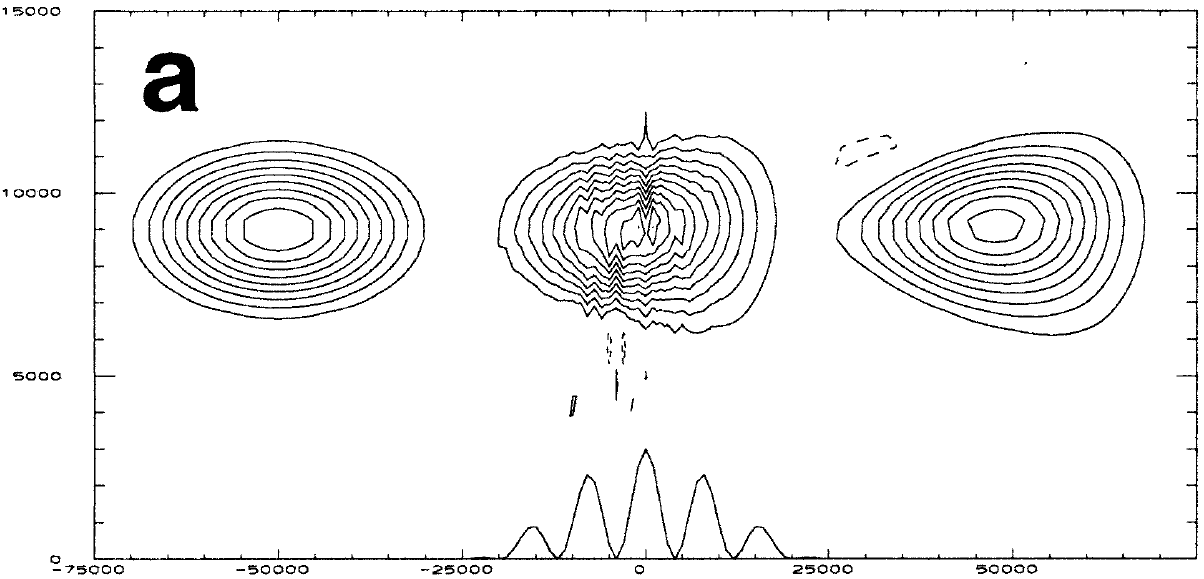
\includegraphics[height=1.2in]{img/schaer-btf-centred.png}}
\\
	\subcaptionbox{SLEVE \label{fig:advection:cubicUpwind:sleve}}[0.49\textwidth]{\input{advection-sleve-schaerCos-cubicUpwindCPCFit-contour-plot}}
	\hfill
	\subcaptionbox{SLEVE from \textcite{schaer2002} \label{fig:advection:schaer:sleve}}[0.49\textwidth]{\vspace{0.43in}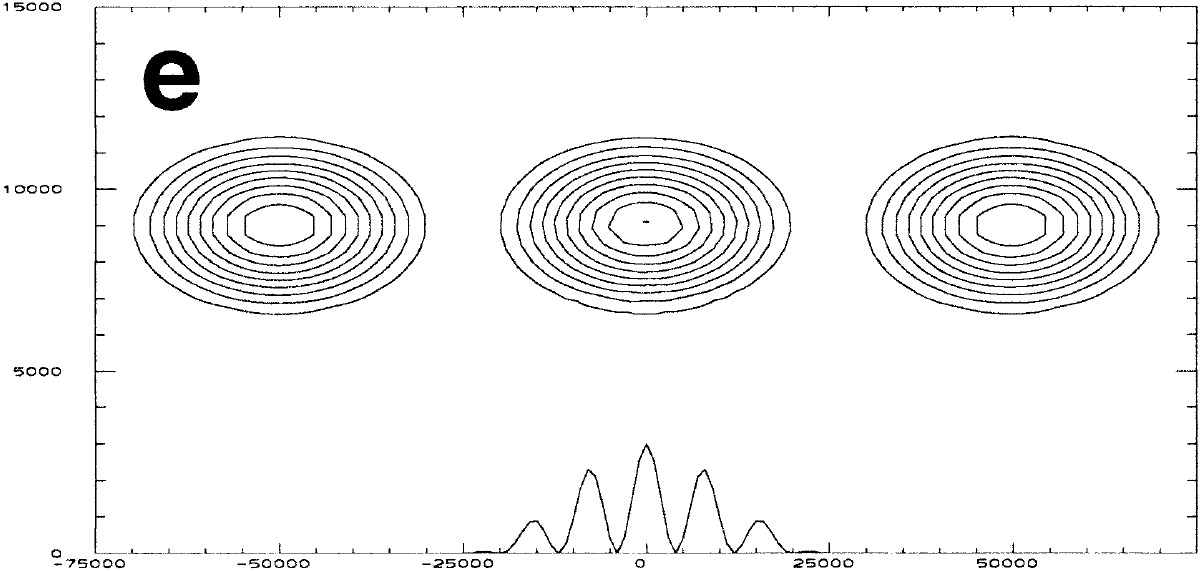
\includegraphics[height=1.2in]{img/schaer-sleve-centred.png}}
\\
	\subcaptionbox{SnapCol grid \label{fig:advection:cubicUpwind:snapCol}}[0.49\textwidth]{\input{advection-snapCol-schaerCos-cubicUpwindCPCFit-contour-plot}}
	\hfill
	\subcaptionbox{Analytic solution on a regular grid \label{fig:advection:analytic}}[0.49\textwidth]{\input{advection-noOrography-analytic-contour-plot}}
%
	\caption{Horizontally advected tracer contours at $t = \SI{0}{\second}$, \SI{5000}{\second} and \SI{10000}{\second}.  Figures (\protect\subref{fig:advection:cubicUpwind:btf}), (\protect\subref{fig:advection:cubicUpwind:sleve}), and (\protect\subref{fig:advection:cubicUpwind:snapCol}) use the upwind-biased scheme described in section~\ref{sec:method:discretisation}.  Figures (\protect\subref{fig:advection:schaer:btf}) and (\protect\subref{fig:advection:schaer:sleve}) show the results of the second-order centred difference scheme from \textcite{schaer2002}.  Contour intervals are every 0.1.}
	\label{fig:advection:cubicUpwind}
\end{figure}

\begin{figure}
	\captionsetup[subfigure]{position=b}
	\centering
	\subcaptionbox{BTF \label{fig:advection:error:btf:cubicUpwind}}[0.49\textwidth]{\includegraphics[width=1.3in,angle=270]{openfoam/cases/advection/btf/schaerCos/cubicUpwindCPCFit/10000/tracer-contour-error.eps}}
	\hfill
	\subcaptionbox{BTF from \textcite{schaer2002} \label{fig:advection:error:schaer:btf}}[0.49\textwidth]{\vspace{0.1in}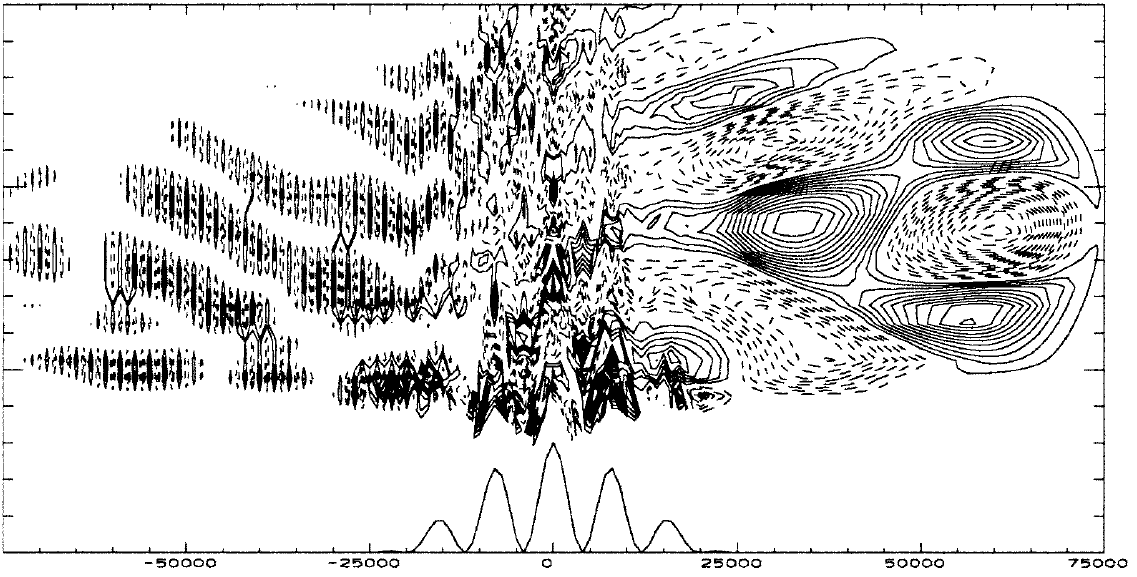
\includegraphics[height=1.2in]{img/schaer-btf-centred-error.png}} \\
%
	\subcaptionbox{SLEVE \label{fig:advection:error:sleve:cubicUpwind}}[0.49\textwidth]{\includegraphics[width=1.3in,angle=270]{openfoam/cases/advection/sleve/schaerCos/cubicUpwindCPCFit/10000/tracer-contour-error.eps}}
	\hfill
	\subcaptionbox{SLEVE from \textcite{schaer2002} \label{fig:advection:error:schaer:sleve}}[0.49\textwidth]{\vspace{0.1in}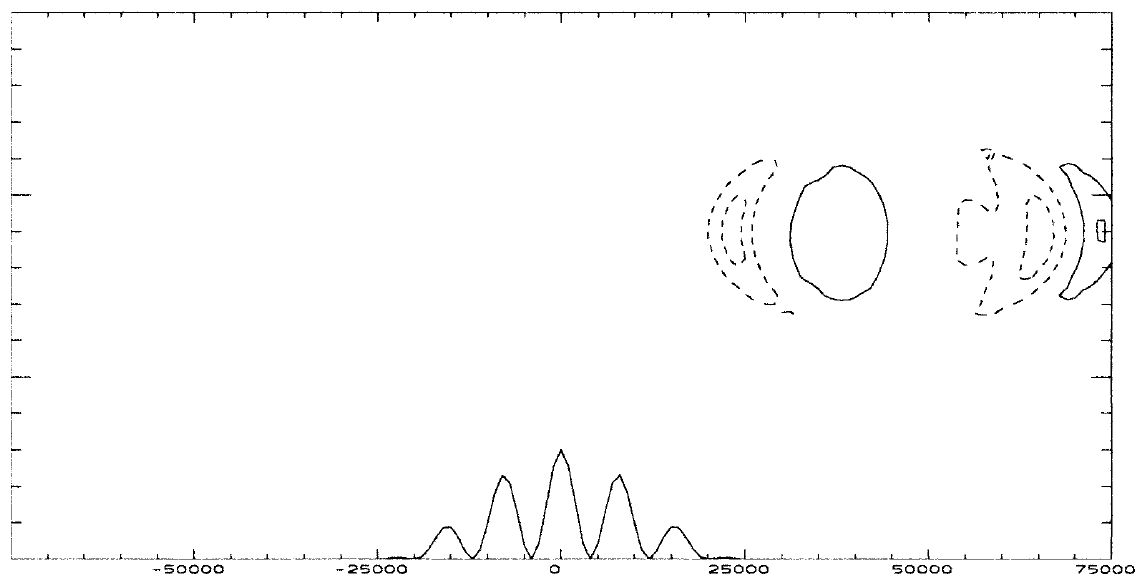
\includegraphics[height=1.2in]{img/schaer-sleve-centred-error.png}} \\
%
	\subcaptionbox{Regular grid \label{fig:advection:error:noOrography:cubicUpwind}}[0.49\textwidth]{\includegraphics[width=1.3in,angle=270]{openfoam/cases/advection/noOrography/cubicUpwindCPCFit/10000/tracer-contour-error.eps}}
	\hfill
	\subcaptionbox{Regular grid from \textcite{schaer2002} \label{fig:advection:error:schaer:noOrography}}[0.49\textwidth]{\vspace{0.1in}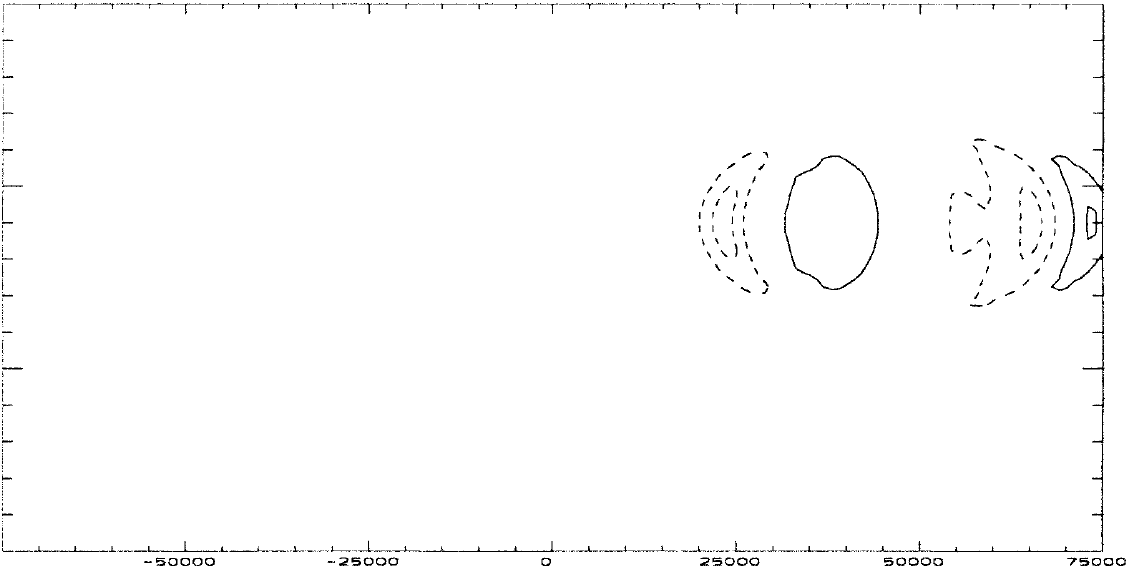
\includegraphics[height=1.2in]{img/schaer-noOrography-centred-error.png}} \\
%
	\caption{Errors in horizontal tracer advection at $t = \SI{10000}{\second}$.  Figures (\protect\subref{fig:advection:error:btf:cubicUpwind}), (\protect\subref{fig:advection:error:sleve:cubicUpwind}) and (\protect\subref{fig:advection:error:noOrography:cubicUpwind}) use the upwind-biased scheme.  Figures (\protect\subref{fig:advection:error:schaer:btf}), (\protect\subref{fig:advection:error:schaer:sleve}) and (\protect\subref{fig:advection:error:schaer:noOrography}) show the error of the second-order centred difference scheme from \textcite{schaer2002}.  Contour intervals are every 0.01, with negative contours denoted by dashed lines.}
	\label{fig:advection:error}
\end{figure}

Results of advection are presented in figure~\ref{fig:advection:cubicUpwind}.
On the BTF grid, the tracer suffers from distortion over the mountain and some artefacts just above the mountain remain as the tracer moves over it.  Comparing figures~\ref{fig:advection:cubicUpwind:btf} and \ref{fig:advection:schaer:btf}, we see that the tracer retains its shape far better than the result from \textcite{schaer2002} that uses a second-order centred difference scheme.  This is expected since the upwind-biased cubic scheme has a larger stencil and higher order accuracy.  Comparing figures~\ref{fig:advection:error:btf:cubicUpwind} and \ref{fig:advection:error:schaer:btf} we see that, unlike the results from \textcite{schaer2002}, errors on the BTF grid are confined to regions around the tracer and near the mountain peak.

As seen in figure~\ref{fig:advection:cubicUpwind:sleve}, results on the SLEVE grid are much closer to the analytic solution on a regular grid (figure~\ref{fig:advection:analytic}).  The tracer retains its shape throughout the simulation and does not suffer from any noticeable distortion.  We find that accuracy is slightly better than the result from \textcite{schaer2002} (see figures~\ref{fig:advection:error:sleve:cubicUpwind} and \ref{fig:advection:error:schaer:sleve}).  Unlike \textcite{schaer2002}, a further improvement in accuracy is seen on a regular grid, as shown in figure~\ref{fig:advection:error:noOrography:cubicUpwind}.

Since the SnapCol grid is entirely regular away from the surface, it is unsurprising that the results (shown in figure~\ref{fig:advection:cubicUpwind:snapCol}) are the same as advection on a regular grid (not shown).  This result agrees with that found by \textcite{good2013}.

At $t = \SI{0}{\second}$, the tracer ranges between zero and one.  Over time, new extrema are generated because the upwind-biased advection scheme is not monotonic.  This is most evident on the BTF grid where the stationary artefacts above the mountain peak reach a minimum of \input{openfoam/cases/advection/btf/schaerCos/cubicUpwindCPCFit/min.txt} by the end of the simulation.  The results of the second-order centred difference scheme of \textcite{schaer2002} show significant negative tracer values as evidenced by the dashed contours in figure~\ref{fig:advection:schaer:btf}.  Minimum values remain close to zero on the SLEVE, SnapCol and regular grids.  All grids show some decrease in maximum tracer magnitude and, once again, the decrease is most severe on the BTF grid.  Results of tracer extrema on all grids are compared to the analytic solution in figure~\ref{fig:wobblyTracerAdvection:ranges:horizontal} and the values are given in table~\ref{tab:advection:errors} on page~\pageref{tab:advection:errors}.

Because the upwind-biased advection scheme is not monotonic, one source of new extrema is a divergent velocity field.  Areas of convergence will increase tracer magnitude and areas of divergence will reduce it.  Although the continuous velocity field in this test is non-divergent, this is not necessarily true of the discrete velocity field, especially where the grid is non-orthogonal.

\begin{figure}
	\centering
	\documentclass[tikz]{standalone}
\usepackage{bm}
\newcommand{\vect}{\bm}
\newcommand{\del}{\nabla}

\begin{document}
\begin{tikzpicture}[
  scale=0.75,
  cpnt/.style={fill=gray},
  vertex/.style={fill=black},
  arr/.style={ultra thick, ->},
  mag/.style={dashed, thick, <->}
]
\draw (0,0) -- (4,0);
\draw (0,3) -- (4,3);
\draw [dashed, thick] (0,0) -- (0,3);
\draw [dashed, thick] (4,0) -- (4,3);
\draw (4,3) -- (8,5) -- (8,2) -- (4,0);
\draw (0,0) -- (-4,-3) -- (-4,0) -- (0,3);
\path [cpnt] (-2,0) circle [radius=0.15] node [above right] {$c_0$};
\path [cpnt] (2,1.5) circle [radius=0.15] node [above right] {$c_1$};
\path [cpnt] (6,2.5) circle [radius=0.15] node [above right] {$c_2$};

\draw (0,1.5) circle [radius=0.15];
\draw (4,1.5) circle [radius=0.15];o

\draw [thick, ->] (-0.5,1.5) -- (0.5,1.5) node [above] {$f_\mathrm{in}$};
\draw [ultra thick, ->] (3,1.5) -- (5,1.5) node [above] {$f_\mathrm{out}$};
\end{tikzpicture}
\end{document}

	\caption{Flux through two faces, shown with dashed lines, in a rectangular cell in the region of vertical wind shear.  Because the surrounding cells are non-orthogonal, interpolation onto cell faces results in a net outward flux which leads to a decrease in tracer magnitude.  Cell centres are denoted by grey circles, face centres are denoted by open circles.}
	\label{fig:advection:flux}
\end{figure}

Let us consider the fluxes in and out of the vertically-oriented faces, $\fin$ and $\fout$, of a rectangular cell in the region of vertical wind shear such that its cell centre $c_1$ has a height $\SI{4}{\kilo\meter} < z < \SI{5}{\kilo\meter}$.  To its left is a cell whose centre, $c_0$, is lower and to its right, a cell whose centre, $c_2$, is higher.  This situation is shown in figure~\ref{fig:advection:flux}.

During model initialisation, the solver interpolates velocities at cell centres onto cell faces, such that $\fin$ is interpolated from $c_0$ and $c_1$, and $\fout$ is an interpolation of $c_1$ and $c_2$.  Remember that horizontal wind is increasing with height, $u(c_2) > u(c_1) > u(c_0)$, and so $\fout > \fin$.  Therefore, there is a net divergence in the rectangular cell, which leads to a decrease in tracer magnitude.

\begin{figure}
	\captionsetup[subfigure]{position=b}
	\centering
	\subcaptionbox{BTF \label{fig:advection:div:btf}}[0.49\textwidth]{\includegraphics[width=1.8in,angle=270]{openfoam/cases/advection/btf/schaerCos/cubicUpwindCPCFit/0/divU.eps}}
	\hfill
	\subcaptionbox{SLEVE \label{fig:advection:div:sleve}}[0.49\textwidth]{\includegraphics[width=1.8in,angle=270]{openfoam/cases/advection/sleve/schaerCos/cubicUpwindCPCFit/0/divU.eps}}
%
	\includegraphics[height=5in,angle=270]{legends/divU.eps}
%
	\caption{\TODO{divergence. don't forget units}}
	\label{fig:advection:div}
\end{figure}

\TODO{now we can talk about how we measured divergence, and the results we got, and what we can conclude from this}

The $\ell^2$ error norms are also summarised in table~\ref{tab:advection:errors}.  Errors on the BTF grid are an order of magnitude greater than the three other grids tested.  The cut cell grid offers only a small error reduction compared to the SLEVE grid.  Even on the BTF grid, the upwind-biased advection scheme is far more tolerant of grid distortions than results of the fourth-order centred scheme from \textcite{schaer2002} (not shown).



\section{Terrain following tracer advection}
\label{sec:wobblyTracerAdvection}

In the horizontal advection test, results were more accurate when the flow was aligned with grid layers: on the cut cell grid results were accurate, but distortions in the BTF grid led to increased error.  This terrain following advection test is designed to determine the nature of these errors by prescribing a velocity field that is aligned with the layers of the BTF grid.  If errors are caused by skewness or grid non-uniformity (described in section~\ref{sec:theory:skewness}), we expect least accuracy on terrain following grids since they are less orthogonal.  However, if errors are caused by flow crossing grid layers, then results are expected to be less accurate on the SnapCol grid.

\subsection{Specification}
The spatial domain, mountain profile, initial tracer profile and discretisation are the same as those in the horizontal tracer advection test (section~\ref{sec:advection}).  The velocity field, however, is defined using a streamfunction $\Psi$ so that the velocity field is non-divergent.  Unlike the horizontal advection test, flow extends from the top of the domain all the way to the ground.  It is defined so that flow is everywhere tangential to BTF coordinate surfaces given by equation~\ref{eqn:theory:btf} such that
\begin{align}
	\Psi(x,z) &= H \frac{z - h}{H - h}
%
	\intertext{The horizontal and vertical components of velocity, $u$ and $w$ are then given by}
%
	u &= \frac{\partial \Psi}{\partial z} \quad,\quad  w = -\frac{\partial \Psi}{\partial x}
%
	\intertext{Hence, for the mountain profile given in equation~\ref{eqn:advection:schaerCos} we find}
%
	u &= \frac{H}{H - h} \quad,\quad w = H \frac{\partial h}{\partial x} \frac{H - z}{\left( H - h \right)^2} \label{eqn:wobblyTracerAdvection:velocity} \\
	\frac{\partial h}{\partial x} &= - h_0 \pi \left[ 
		\frac{1}{\lambda} \cos^2 \left( \frac{\pi x}{2a} \right) \sin \left( \frac{2 \pi x}{\lambda} \right) +
		\frac{1}{2a} \cos^2 \left( \frac{\pi x}{\lambda} \right) \sin \left( \frac{\pi x}{a} \right)
	\right]
\end{align}
The resulting velocity field is shown in figure~\ref{fig:wobblyTracer:u}.

\begin{figure}
	\centering
	\includegraphics[width=2.0in,angle=270]{openfoam/cases/wobblyTracerAdvection/btf/schaerCos/cubicUpwindCPCFit/0/U.eps}
	\TODO{also plot flow on snapCol grid?}
%
	\caption{Terrain following velocity field with flow everywhere tangential to BTF coordinate surfaces.  Outline of BTF grid shown in grey.  Only the lowest \SI{15}{\kilo\meter} of the central \SI{60}{\kilo\meter} is shown.  The entire domain is \SI{300}{\kilo\meter} wide and \SI{25}{\kilo\meter} high.}
	\label{fig:wobblyTracer:u}
\end{figure}

\subsection{Analysis}

\begin{figure}
	\captionsetup[subfigure]{position=b}
	\centering
	\subcaptionbox{BTF \label{fig:wobblyTracerAdvection:btf}}[0.49\textwidth]{\input{wobblyTracerAdvection-btf-schaerCos-cubicUpwindCPCFit-contour-plot}}
	\hfill
	\subcaptionbox{SnapCol \label{fig:wobblyTracerAdvection:snapCol}}[0.49\textwidth]{\input{wobblyTracerAdvection-snapCol-schaerCos-cubicUpwindCPCFit-contour-plot}}
%
	\caption{Advected tracer contours in a terrain following velocity field at $t = \SI{0}{\second}$, \SI{5000}{\second} and \SI{10000}{\second}.  Contour intervals are every 0.1.}
\end{figure}

Accuracy increases on the BTF grid compared to the horizontal tracer advection test: artefacts above the mountain, as seen in figure~\ref{fig:advection:cubicUpwind:btf}, are no longer present in figure~\ref{fig:wobblyTracerAdvection:btf}.  This is confirmed by the absence of the large magnitude negative tracer, as shown in figure~\ref{fig:wobblyTracerAdvection:ranges}.  The $\ell^2$ error norm is reduced from \input{openfoam/cases/advection/btf/schaerCos/cubicUpwindCPCFit/l2error.txt} to \input{openfoam/cases/wobblyTracerAdvection/btf/schaerCos/cubicUpwindCPCFit/l2error.txt}\unskip.  Despite the large distortions due to the oscillating velocity field above the mountain, tracer shape is preserved having cleared the mountain at $t = \SI{10000}{\second}$.

In contrast, the tracer suffers from significantly reduced accuracy on the SnapCol grid as evidenced by the fewer, wider contours in figure~\ref{fig:wobblyTracerAdvection:snapCol}.  Accuracy on the SnapCol grid is lower than that for any other tracer advection.  Tracer amplitude is reduced to \input{openfoam/cases/wobblyTracerAdvection/snapCol/schaerCos/cubicUpwindCPCFit/max.txt} (see figure~\ref{fig:wobblyTracerAdvection:ranges:tf}).  $\ell^2$ error norms are compared with those for horizontal advection in table~\ref{tab:advection:errors}.

\begin{figure}
	\captionsetup[subfigure]{position=b}
	\centering
%
	\subcaptionbox{BTF \label{fig:wobblyTracerAdvection:div:btf}}[0.49\textwidth]{\includegraphics[width=1.8in,angle=270]{openfoam/cases/wobblyTracerAdvection/btf/schaerCos/cubicUpwindCPCFit/0/divU.eps}}
	\hfill
	\subcaptionbox{SnapCol \label{fig:wobblyTracerAdvection:div:snapCol}}[0.49\textwidth]{\includegraphics[width=1.8in,angle=270]{openfoam/cases/wobblyTracerAdvection/snapCol/schaerCos/cubicUpwindCPCFit/0/divU.eps}}
%
	\includegraphics[height=5in,angle=270]{legends/divU.eps}
%
	\caption{Divergence (\si{\per\second}) of the discrete velocity field in the centremost \SI{20}{\kilo\meter} and lowest \SI{8}{\kilo\meter} on (\subcaptionref{fig:wobblyTracerAdvection:div:btf}) the BTF grid, and (\subcaptionref{fig:wobblyTracerAdvection:div:snapCol}) the SnapCol grid.}
	\label{fig:wobblyTracerAdvection:div}
\end{figure}

\TODO{discuss (lack of) divergence in this test.}

Given these results, we conclude that advection errors are mainly due to lack of flow alignment rather than skewness or grid non-uniformity.

\begin{figure}
	\captionsetup[subfigure]{position=b}
	\centering
	\subcaptionbox{Horizontal advection \label{fig:wobblyTracerAdvection:ranges:horizontal}}[\textwidth]{\input{advection-tracer-range-plot}} \\
	\subcaptionbox{Terrain following advection \label{fig:wobblyTracerAdvection:ranges:tf}}[\textwidth]{\input{wobblyTracerAdvection-tracer-range-plot}}
%
	\caption{Comparison of minimum and maximum tracer values at $t = \SI{10000}{\second}$ for horizontal and terrain following tracer advection tests.  Initially, tracer magnitude ranges from zero to one.}
	\label{fig:wobblyTracerAdvection:ranges}
\end{figure}

\begin{table}
\centering
\begin{tabular}{ r @{\hspace{2em}} l l l l l l}
\toprule
		& \multicolumn{2}{c}{$\ell^2$ error norm} & \multicolumn{2}{c}{Minimum} & \multicolumn{2}{c}{Maximum} \\
		& Horizontal & TF & Horizontal & TF & Horizontal & TF \\ \midrule
Analytic & 0 & 0 & 0 & 0 & 1 & 1 \\
BTF
	& \input{openfoam/cases/advection/btf/schaerCos/cubicUpwindCPCFit/l2error.txt}
	& \input{openfoam/cases/wobblyTracerAdvection/btf/schaerCos/cubicUpwindCPCFit/l2error.txt}
	& \input{openfoam/cases/advection/btf/schaerCos/cubicUpwindCPCFit/min.txt}
	& \input{openfoam/cases/wobblyTracerAdvection/btf/schaerCos/cubicUpwindCPCFit/min.txt}
	& \input{openfoam/cases/advection/btf/schaerCos/cubicUpwindCPCFit/max.txt}
	& \input{openfoam/cases/wobblyTracerAdvection/btf/schaerCos/cubicUpwindCPCFit/max.txt} \\
SLEVE
	& \input{openfoam/cases/advection/sleve/schaerCos/cubicUpwindCPCFit/l2error.txt}
	& ---
	& \input{openfoam/cases/advection/sleve/schaerCos/cubicUpwindCPCFit/min.txt}
	& ---
	& \input{openfoam/cases/advection/sleve/schaerCos/cubicUpwindCPCFit/max.txt}
	& --- \\
SnapCol
	& \input{openfoam/cases/advection/snapCol/schaerCos/cubicUpwindCPCFit/l2error.txt}
	& \input{openfoam/cases/wobblyTracerAdvection/snapCol/schaerCos/cubicUpwindCPCFit/l2error.txt}
	& \input{openfoam/cases/advection/snapCol/schaerCos/cubicUpwindCPCFit/min.txt}
	& \input{openfoam/cases/wobblyTracerAdvection/snapCol/schaerCos/cubicUpwindCPCFit/min.txt}
	& \input{openfoam/cases/advection/snapCol/schaerCos/cubicUpwindCPCFit/max.txt}
	& \input{openfoam/cases/wobblyTracerAdvection/snapCol/schaerCos/cubicUpwindCPCFit/max.txt} \\
Regular grid
	& \input{openfoam/cases/advection/noOrography/cubicUpwindCPCFit/l2error.txt}
	& ---
	& \input{openfoam/cases/advection/noOrography/cubicUpwindCPCFit/min.txt}
	& ---
	& \input{openfoam/cases/advection/noOrography/cubicUpwindCPCFit/max.txt}
	& --- \\ \bottomrule
\end{tabular}
%
\caption{$\ell^2$ error norms, minimum and maximum tracer values for the horizontal and terrain following tracer advection tests at $t = \SI{10000}{\second}$.  Horizontal tracer advection is discussed in section~\ref{sec:advection}, terrain following advection in section~\ref{sec:wobblyTracerAdvection}, and only tested on BTF and SnapCol grids.}
\label{tab:advection:errors}
\end{table}


\section{Resting atmosphere}
\label{sec:resting}

This two-dimensional test simulates a stably stratified atmosphere in hydrostatic balance.  Since there are no net forces, the analytical solution should remain at rest.  The test specification follows that from \textcite{klemp2011}, and challenges the accuracy of the calculation of the horizontal pressure gradient.  An inversion layer causes nonlinear processes that further tax the model \autocite{good2013}.

\subsection{Specification}
Following \textcite{weller-shahrokhi2014}, the domain is \SI{20}{\kilo\meter} wide and \SI{20}{\kilo\meter} high, which is narrower than \textcite{klemp2011} in order to reduce simulation time.  The wave-shaped mountain profile is taken from \textcite{schaer2002} where the surface height $h$ is given by
\begin{align}
	\surface(x) = \surface_0 \exp \left( - \left( \frac{x}{a} \right)^2 \right) \cos^2 \left( \frac{\pi x}{\lambda} \right) \label{eqn:resting:mountain}
\end{align}
where $a = \SI{5}{\kilo\meter}$ is the mountain half-width, $h_0 = \SI{1}{\kilo\meter}$ is the maximum mountain height and $\lambda = \SI{4}{\kilo\meter}$ is the wavelength.  For the optimised SLEVE grid, the large-scale component $\surface_1$, described in section~\ref{sec:theory:tf}, is specified as
\begin{align}
\surface_1(x) = \frac{1}{2} \surface_0 \exp \left( - \left( \frac{x}{a} \right)^2 \right)
\end{align}
and, following \cite{leuenberger2010}, $s_1 = \SI{4}{\kilo\meter}$ is the large scale height, $s_2 = \SI{1}{\kilo\meter}$ is the small scale height, and the optimal exponent value of $n = 1.35$ is used.  Results are compared with the numerical solution with no orography.

The initial thermodynamic conditions have a surface temperature of $\theta_0 = \SI{288}{\kelvin}$ and constant stability with Brunt-V\"ais\"al\"a frequency $N = \SI{0.01}{\per\second}$ everywhere, except for a more stable layer of $N = \SI{0.02}{\per\second}$ between $\SI{2}{\kilo\meter} \leq z \leq \SI{3}{\kilo\meter}$.

\subsection{Diagnostics}
Two metrics were used to measure the model error.  First, maximum vertical velocity is measured at each timestep.  An analytic solution has no vertical velocity $w$ since the atmosphere is at rest.  However, numerical error in calculating the horizontal pressure gradient give rise to spurious vertical velocities which become more severe over steep terrain \autocite{klemp2011}.

Second, normalised energy change $\Delta E$ is measured for each timestep as described in section~\ref{sec:method:energy}.  The total normalised energy change is the sum of normalised kinetic, potential, and internal energy changes.
An analytic solution would conserve total energy such that $\Delta E(t) = 0\;\forall\;t$.  As discussed in \textcite{weller-shahrokhi2014}, energy is not exactly conserved in the model presented because of damping by the advection scheme and inexact transfer between kinetic, internal and potential energy.

\subsection{Discretisation}
The simulation uses the discretisation of the fully-compressible Euler equations described in section~\ref{sec:method:discretisation}.  The domain is discretised on a grid having $40 \times 40$ cells such that $\Delta x = \Delta z = \SI{0.5}{\kilo\meter}$.  All boundary conditions are no normal flow.  The simulation is integrated forward by 5 hours with a timestep $\Delta t = \SI{100}{\second}$.  Unlike \textcite{klemp2011}, there is no eddy diffusion in the equation set.

\subsection{Results}
\begin{figure}
	\captionsetup[subfigure]{position=b}
	\centering
	\subcaptionbox{Model results \label{fig:resting:w:model}}[0.58\textwidth]{\input{resting-w-plot}}
	\hfill
	\subcaptionbox{Results from \textcite{klemp2011}}[0.4\textwidth]{\vspace{0.27in}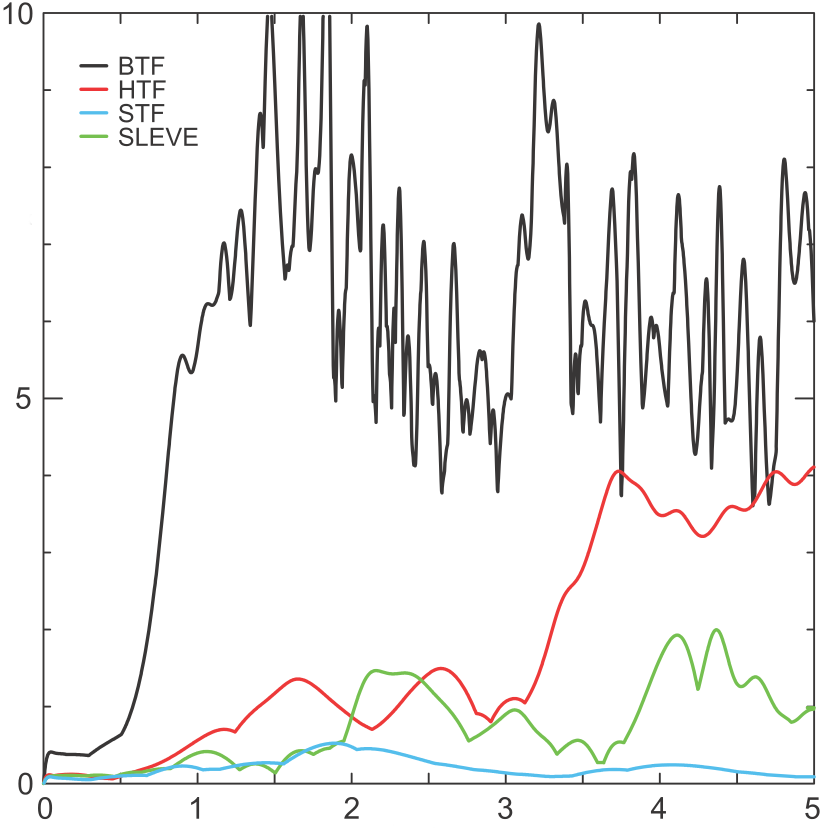
\includegraphics[height=2in]{img/klemp-w.png}}
	\caption{Maximum spurious vertical velocity $w$ in the resting atmosphere test compared with results from \textcite{klemp2011}.  Note that vertical scales differ.}
	\label{fig:resting:w}
\end{figure}

Test results for BTF, optimised SLEVE, and SnapCol grids are compared with results on a regular grid with no orography.  On the BTF grid, spurious vertical velocity $w$ reaches $\sim \SI{0.35}{\meter\per\second}$, which is significantly less than the velocities of $\sim \SI{10}{\meter\per\second}$ found by \textcite{klemp2011} (see figure~\ref{fig:resting:w}, note different vertical scales).  An oscillation develops after 4 hours, the cause of which is not yet known.  Unlike the results from \textcite{klemp2011}, the optimised SLEVE grid does not significantly reduce $w$ compared to BTF.  Since the model and its initialisation are the same, results on the BTF and optimised SLEVE grids are also in agreement with \textcite{weller-shahrokhi2014}.

The SnapCol grid results in a significantly smaller maximum vertical velocity of less than \SI{1e-3}{\meter\per\second}.  The smallest error of $\sim \SI{1e-10}{\meter\per\second}$ is found on the regular grid.  This error may be due to loss of precision when OpenFOAM loads the initial conditions, which are in discrete hydrostatic balance, but the source of the error is not certain.

\begin{figure}
	\captionsetup[subfigure]{position=b}
	\centering
	\subcaptionbox{Cell centres at centre of uncut cells leading to some cell centres below the ground \label{fig:resting:good:uncut}}[0.49\textwidth]{\input{resting-good-uncut-plot}}
	\hfill
	\subcaptionbox{Cell centres at centre of cut cells \label{fig:resting:good:cut}}[0.49\textwidth]{\input{resting-good-cut-plot}}
%
	\caption{Placement of cell centres on a two-dimensional cut cell grid.  The model from \textcite{good2013} has some cell centres below the ground (B. Good 2014, personal communication).  The arrows denote an estimated horizontal gradient between two adjacent cells of a scalar value stored at cell centres.}
	\label{fig:resting:good}
\end{figure}

Using a timestep of \SI{1.01}{\second}, \textcite{good2013} found the maximum vertical velocity in their cut cell model was \SI{1e-12}{\meter\per\second}, which is better than any result from the experiments in this project.  However, in that model, cell centres are in the centre of the uncut cell, resulting in the centre of some cut cells being below the ground, as shown in figure~\ref{fig:resting:good} (B. Good 2014, personal communication).  This means that the grid is effectively regular when calculating horizontal and vertical gradients.

\begin{figure}
	\captionsetup[subfigure]{position=b}
	\centering
	\subcaptionbox{Total normalised energy changes on terrain following grids \label{fig:resting:energy:total-tf}}[0.32\textwidth]{\input{resting-energy-total-tf-plot}}
	\hfill
	\subcaptionbox{As (\subcaptionref{fig:resting:energy:total-tf}), but on the SnapCol grid \label{fig:resting:energy:total-snapCol}}[0.32\textwidth]{\input{resting-energy-total-snapCol-plot}}
	\hfill
	\subcaptionbox{As (\subcaptionref{fig:resting:energy:total-tf}), but on a regular grid with no orography \label{fig:resting:energy:total-noOrography}}[0.32\textwidth]{\input{resting-energy-total-noOrography-plot}}
	\\
	\subcaptionbox{Kinetic ($E_K$), potential ($E_P$) and internal ($E_I$) normalised energy changes on BTF grid \label{fig:resting:energy:btf}}[0.32\textwidth]{\input{resting-energy-btf-plot}}
	\hfill
	\subcaptionbox{As (\subcaptionref{fig:resting:energy:btf}), but on the optimised SLEVE grid \label{fig:resting:energy:sleve}}[0.32\textwidth]{\input{resting-energy-sleve-plot}}
	\hfill
	\subcaptionbox{As (\subcaptionref{fig:resting:energy:btf}), but on the SnapCol grid.  Note the different vertical scale from figures~(\subcaptionref{fig:resting:energy:btf}) and (\subcaptionref{fig:resting:energy:sleve}). \label{fig:resting:energy:snapCol}}[0.32\textwidth]{\input{resting-energy-snapCol-plot}}
	\caption{Comparison of normalised energy changes on BTF, optimised SLEVE and SnapCol grids for the resting atmosphere test.}
	\label{fig:resting:energy}
\end{figure}

Examining normalised energy change, shown in figure~\ref{fig:resting:energy:total-tf}, we find that there is a net loss of energy on BTF and optimised SLEVE grids.  However, there is a period of energy gain on the optimised SLEVE grid during the first two hours, and an upward trend in energy after 3 hours on the BTF grid.  The cause of the energy gain is the subject of further work (see chapter~\ref{sec:further-work}).

Energy is better conserved on the SnapCol grid, the energy loss being more than two orders of magnitude smaller than the terrain following grids (figure~\ref{fig:resting:energy:total-snapCol}).  This compares favourably with the best possible energy conservation for this model as found on a regular grid (figure~\ref{fig:resting:energy:total-noOrography}).

The spurious motion generated by horizontal pressure gradient errors leads to a positive change in kinetic energy, evident in figures~\ref{fig:resting:energy:btf} and~\ref{fig:resting:energy:sleve}.  Compared to both terrain following grids, internal and potential energy conservation is three orders of magnitude better on the SnapCol grid (\ref{fig:resting:energy:snapCol}).  As noted by \textcite{weller-shahrokhi2014}, the model converts between potential and internal energy on timescales of less than an hour.  This can be seen by the mirroring between $E_P$ and $E_I$ plots, and we confirm that this local energy conservation property is present in all three grids (figures~\ref{fig:resting:energy:btf}, \subcaptionref{fig:resting:energy:sleve} and \subcaptionref{fig:resting:energy:snapCol}).

\TODO{if I want to compare to Zaengl (and also Good), I would need to try the same experiment with 4km high mountain, too}

\TODO{I could compare theta field (as done by Klemp)}


\section{Gravity waves}
\label{sec:gw}

Following \textcite{schaer2002}, uniform flow over an idealised two-dimensional mountain ridge induces gravity waves in a stable atmosphere.  As described in section~\ref{sec:theory:gw}, large-scale waves propagate away from the surface and small-scale evanescent waves decay rapidly above the terrain.

\subsection{Specification}
Following \textcite{melvin2010}, the domain is \SI{300}{\kilo\meter} wide and \SI{30}{\kilo\meter} high.  The mountain profile has the same form as equation~\ref{eqn:resting:mountain} but with a lower maximum height of $\surface_0 = \SI{250}{\meter}$.  As in the resting atmosphere test, $a = \SI{5}{\kilo\meter}$ is the mountain half-width and $\lambda = \SI{4}{\kilo\meter}$ is the wavelength.  On the optimised SLEVE grid, $s_1 = \SI{5}{\kilo\meter}$ is the large scale height, $s_2 = \SI{2}{\kilo\meter}$ is the small scale height and the optimal exponent value $n = 1.35$ as in the previous test.

The initial thermodynamic conditions have a surface temperature of $\theta_0 = \SI{288}{\kelvin}$ and constant stability with $N = \SI{0.01}{\per\second}$ everywhere.  A constant horizontal wind $u = \SI{10}{\meter\per\second}$ is prescribed at the inlet boundary.

\subsection{Discretisation}
The test uses the discretisation of the Euler equations described in section~\ref{sec:method:discretisation}.  The domain is discretised on a grid having $600 \times 100$ cells such that $\Delta x = \SI{0.5}{\kilo\meter}$ and $\Delta z = \SI{300}{\meter}$.  Sponge layers are added to the upper \SI{10}{\kilo\meter} and leftmost \SI{10}{\kilo\meter} at the inlet boundary to damp the reflection of waves.
The term $\mu \rho \vect{u}$ is subtracted from the momentum equation (equation~\ref{eqn:method:momentum}) where the damping function $\mu$ is adapted from \textcite{melvin2010} such that
\begin{align}
	\mu(x, z) &= \mu_\mathrm{upper} + \mu_\mathrm{inlet} \\
	\mu_\mathrm{upper}(z) &= \begin{cases}
		\overline{\mu} \sin^2 \left( \frac{\pi}{2} \frac{z - z_B}{H - z_B} \right) & \text{if } z \geq z_B \\
		0 & \text{otherwise} \\
	\end{cases} \\
	\mu_\mathrm{inlet}(x) &= \begin{cases}
		\overline{\mu} \sin^2 \left( \frac{\pi}{2} \frac{x_I - x}{x_I - x_0} \right) & \text{if } x < x_I \\
		0 & \text{otherwise}
	\end{cases}
\end{align}
where $\overline{\mu} = 1.2$ is the damping coefficient, $z_B = \SI{20}{\kilo\meter}$ is the bottom of the sponge layer, $H = \SI{30}{\kilo\meter}$ is the top of the domain, $x_0 = \SI{-150}{\kilo\meter}$ is the leftmost limit of the domain and $x_I = \SI{-140}{\kilo\meter}$ is the rightmost extent of the inlet sponge layer.  The sponge layer is only active on faces whose normal is vertical so that it damps vertical momentum only.

Note that, while the domain itself is \SI{30}{\kilo\meter} in height, for the purposes of generating of BTF and SLEVE grids, the domain height is set to \SI{20}{\kilo\meter} because the sponge layer occupies the uppermost \SI{10}{\kilo\meter}.

No slip conditions are imposed on the top and bottom boundaries and the outlet is zero gradient.  For Exner, hydrostatic balance is prescribed on all boundaries.  Following \textcite{melvin2010}, the simulation is integrated forward by 5 hours with a timestep $\Delta t = \SI{8}{\second}$.

\subsection{Analysis}

\begin{figure}
	\centering
	\begin{subfigure}[b]{0.48\textwidth}
		\includegraphics[height=2.6in,angle=270]{data/gravityWaves-btf-schaerExp-h/18000/w.eps}\vspace{2em}
		\caption{BTF}
		\label{fig:gw:w:btf}
	\end{subfigure}
	\hfill
	\begin{subfigure}[b]{0.48\textwidth}
		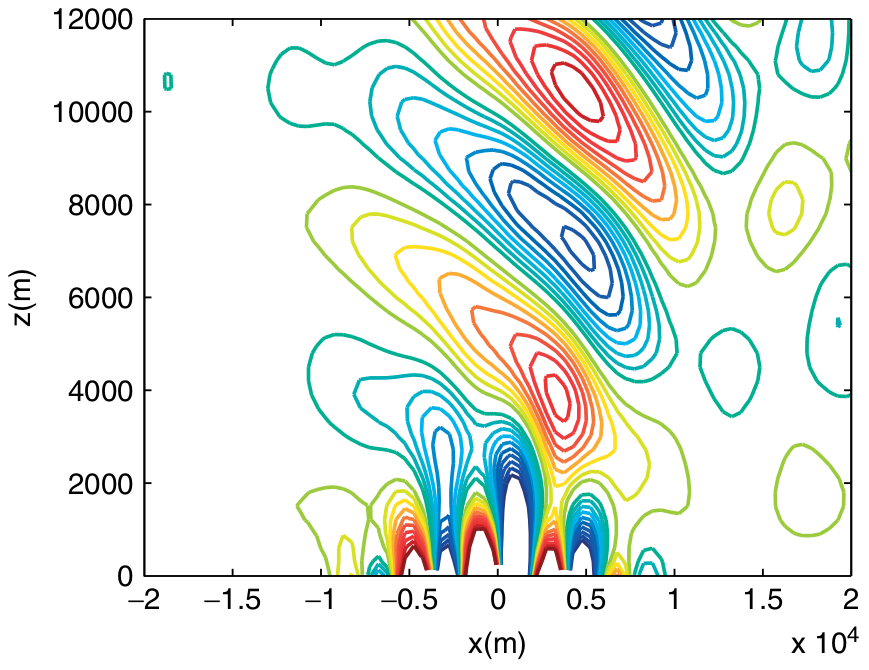
\includegraphics[height=2in]{img/melvin-7a.png}
		\caption{Mass-conserving semi-implicit semi-Lagrangian solution from \textcite{melvin2010}}
		\label{fig:gw:w:melvin}
	\end{subfigure} \\
%
	\begin{subfigure}[b]{0.48\textwidth}
		\includegraphics[height=2.6in,angle=270]{data/gravityWaves-sleve-schaerExp-h/18000/w.eps}
		\caption{SLEVE}
		\label{fig:gw:w:sleve}
	\end{subfigure}
	\hfill
	\begin{subfigure}[b]{0.48\textwidth}
		\includegraphics[height=2.6in,angle=270]{data/gravityWaves-sleve-schaerExp-h/18000/thetaDiff.eps}
		\caption{SLEVE}
		\label{fig:gw:thetaDiff:sleve}
	\end{subfigure} \\
%
	\begin{subfigure}[b]{0.48\textwidth}
		\includegraphics[height=2.6in,angle=270]{data/gravityWaves-sleve-schaerExp-h/18000/w.eps}\vspace{3em}
		\caption{SnapCol}
		\label{fig:gw:w:snapCol}
	\end{subfigure}
	\hfill
	\begin{subfigure}[b]{0.48\textwidth}
		\shortstack[c]{\includegraphics[height=2.6in,angle=270]{data/gravityWaves-snapCol-schaerExp-h/18000/thetaDiff.eps} \\
			\smallskip \hspace{1em} \includegraphics[height=2.4in,angle=270]{legends/thetaDiff.eps}}
		\caption{SnapCol}
		\label{fig:gw:thetaDiff:snapCol}
	\end{subfigure}
%
	\caption{Vertical cross section of vertical velocity contours (\subcaptionref{fig:gw:w:btf}, \subcaptionref{fig:gw:w:sleve} and \subcaptionref{fig:gw:w:snapCol}) and potential temperature anomalies in Kelvin (\subcaptionref{fig:gw:thetaDiff:sleve} and \subcaptionref{fig:gw:thetaDiff:snapCol}) from the gravity waves test after 5 hours.  Vertical velocity contours are every \SI{5e-2}{\meter\per\second} with solid lines denoting ascent and dashed lines descent.}
	\label{fig:gw:w}
\end{figure}

Comparing vertical velocity contours between BTF and SLEVE show few visible differences (figures~\ref{fig:gw:w:btf}, \subcaptionref{fig:gw:w:sleve}).  Evanescent waves are visible as dense contours immediately above the mountain ridges and the large-scale hydrostatic waves propagate vertically.  We verify the two wave types using the linear theory discussed in section~\ref{sec:theory:gw}.  The horizontal wavelength between each mountain peak is specified as $\lambda = \SI{4e3}{\meter}$, so $k = 2 \pi / \lambda \approx \SI{1.57e-3}{\per\meter}$.  The condition for evanescent waves is that $| \overline{u}k | \geq N$.  Since this test specifies $N = \SI{0.01}{\per\second}$ and $\overline{u} = \SI{10}{\meter\per\second}$, we find that the condition is satisfied.

The mountain half-width is specified to be $a = \SI{5e3}{\meter}$, so the large-scale wavelength is \SI{1e4}{\meter} and the horizontal wavenumber $k \approx \SI{6.28e-4}{\per\meter}$.  In this case, $| \overline{u}k | < N$, so waves propagate vertically.  Hence, we have shown that both propagating and evanescent waves are generated by this particular configuration of stability, wind speed, and mountain profile.

Since the same model was used, vertical velocities match those from \textcite{weller-shahrokhi2014}.  Vertical velocities on the SnapCol grid are similar to the terrain following results (figure~\ref{fig:gw:w:snapCol}).  All three results are in agreement with a semi-implicit, semi-Lagrangian simulation from \textcite{melvin2010} (see figure~\ref{fig:gw:w:melvin}).

\begin{figure}
	\captionsetup[subfigure]{position=b}
	\centering
	\subcaptionbox{BTF (gravity waves test) \label{fig:gw:flow:btf}}[0.49\textwidth]{\includegraphics[width=1.5in,angle=270]{data/gravityWaves-btf-schaerExp-h/18000/UfZoom.eps}}
	\subcaptionbox{SnapCol (gravity waves test) \label{fig:gw:flow:snapCol}}[0.49\textwidth]{\includegraphics[width=1.5in,angle=270]{data/gravityWaves-snapCol-schaerExp-h/18000/UfZoom.eps}} \\
%
	\subcaptionbox{BTF (thermal advection test) \label{fig:wobblyThetaAdvection:flow:btf}}[0.49\textwidth]{\includegraphics[width=1.5in,angle=270]{openfoam/cases/wobblyThetaAdvection/btf/schaerExp/cubicUpwindCPCFit/0/Uzoom.eps}}
	\subcaptionbox{SnapCol (thermal advection test) \label{fig:wobblyThetaAdvection:flow:snapCol}}[0.49\textwidth]{\includegraphics[width=1.5in,angle=270]{openfoam/cases/wobblyThetaAdvection/snapCol/schaerExp/cubicUpwindCPCFit/0/Uzoom.eps}} \\
%
	\caption{Vertical cross section of velocity vectors in the centremost \SI{10}{\kilo\meter} and lowest \SI{1.2}{\kilo\meter}.  In the gravity waves test, the velocity field after 5 hours follows the terrain and is qualitatively similar on (\subcaptionref{fig:gw:flow:btf}) the BTF grid, (\subcaptionref{fig:gw:flow:snapCol}) the SnapCol grid, and the SLEVE grid (not shown).  For the thermal advection test described in section~\ref{sec:wobblyThetaAdvection}, the terrain following velocity field is prescribed.  It is designed to imitate the velocity field of the gravity waves test, and is shown here on the BTF grid (\subcaptionref{fig:wobblyThetaAdvection:flow:btf}) and SnapCol grid (\subcaptionref{fig:wobblyThetaAdvection:flow:snapCol}).}
	\label{fig:gw:flow}
\end{figure}

Examining the velocity vector field we find that the flow is qualitatively similar between the BTF grid (figure~\ref{fig:gw:flow:btf}), SnapCol grid (figure~\ref{fig:gw:flow:snapCol}), and SLEVE grid (not shown).  Flow near the ground follows the terrain, accelerating as it passes over the mountain peaks, with velocities becoming more horizontal aloft.  

\begin{figure}
	\captionsetup[subfigure]{position=b}
	\centering
	%
	\subcaptionbox{BTF $h_0 = \SI{250}{\meter}$ \label{fig:gw:div:btf}}[0.49\textwidth]{\includegraphics[width=1.8in,angle=270]{data/gravityWaves-btf-schaerExp-h/18000/divUf.eps}}
	\hfill
	\subcaptionbox{BTF $h_0 = \SI{500}{\meter}$ \label{fig:gw:div:btf-dh}}[0.49\textwidth]{\includegraphics[width=1.8in,angle=270]{data/gravityWaves-btf-schaerExp-doubleHigh-h/18000/divUf.eps}} \\
%
	\subcaptionbox{SLEVE $h_0 = \SI{250}{\meter}$ \label{fig:gw:div:sleve}}[0.49\textwidth]{\includegraphics[width=1.8in,angle=270]{data/gravityWaves-sleve-schaerExp-h/18000/divUf.eps}}
	\hfill
	\subcaptionbox{SLEVE $h_0 = \SI{500}{\meter}$ \label{fig:gw:div:sleve-dh}}[0.49\textwidth]{\includegraphics[width=1.8in,angle=270]{data/gravityWaves-sleve-schaerExp-doubleHigh-h/18000/divUf.eps}} \\
%
	\subcaptionbox{SnapCol $h_0 = \SI{250}{\meter}$ \label{fig:gw:div:snapCol}}[0.49\textwidth]{\includegraphics[width=1.8in,angle=270]{data/gravityWaves-snapCol-schaerExp-h/18000/divUf.eps}}
	\hfill
	\subcaptionbox{SnapCol $h_0 = \SI{500}{\meter}$ \label{fig:gw:div:snapCol-dh}}[0.49\textwidth]{\includegraphics[width=1.8in,angle=270]{data/gravityWaves-snapCol-schaerExp-doubleHigh-h/18000/divUf.eps}} \\
%
	\includegraphics[height=5in,angle=270]{legends/divU.eps}
%
	\caption{Divergence (\si{\per\second}) of the discrete velocity field in the centremost \SI{20}{\kilo\meter} and lowest \SI{8}{\kilo\meter} for a mountain height of $h_0 = \SI{250}{\meter}$ on the BTF grid (\subcaptionref{fig:gw:div:btf}), SLEVE grid (\subcaptionref{fig:gw:div:sleve}), and SnapCol grid (\subcaptionref{fig:gw:div:snapCol}), and for a mountain height of $h_ = \SI{500}{\meter}$ on the BTF, SLEVE and SnapCol grids (\subcaptionref{fig:gw:div:btf-dh}, \subcaptionref{fig:gw:div:sleve-dh} and \subcaptionref{fig:gw:div:snapCol-dh} respectively).}
	\label{fig:gw:div}
\end{figure}

As shown in figure~\ref{fig:gw:div:btf}, \ref{fig:gw:div:sleve} and \ref{fig:gw:div:snapCol}, divergence in the velocity field was found to be negligible everywhere except the lowest layer on all grids.  Magnitude of divergence is slightly greater on the SnapCol grid.

\begin{figure}
	\captionsetup[subfigure]{position=b}
	\centering
	\subcaptionbox{SLEVE $\surface_0 = \SI{250}{\meter}$ \label{fig:gw:thetaDiffZoom:sleve}}[\textwidth]{\includegraphics[width=1.4in,angle=270]{data/gravityWaves-sleve-schaerExp-h/18000/nonlinearMomentumZoom.eps}} \\
	\subcaptionbox{SnapCol $\surface_0 = \SI{250}{\meter}$ \label{fig:gw:thetaDiffZoom:snapCol}}[\textwidth]{\includegraphics[width=1.4in,angle=270]{data/gravityWaves-snapCol-schaerExp-h/18000/nonlinearMomentumZoom.eps}} \\
	\subcaptionbox{SLEVE $\surface_0 = \SI{500}{\meter}$ \label{fig:gw:thetaDiffZoom:sleve-dh}}[\textwidth]{\includegraphics[width=1.4in,angle=270]{data/gravityWaves-sleve-schaerExp-doubleHigh-h/18000/nonlinearMomentumZoom.eps}} \\
	\subcaptionbox{SnapCol $\surface_0 = \SI{500}{\meter}$ \label{fig:gw:thetaDiffZoom:snapCol-dh}}[\textwidth]{\includegraphics[width=1.4in,angle=270]{data/gravityWaves-snapCol-schaerExp-doubleHigh-h/18000/nonlinearMomentumZoom.eps}} \\
%
	\includegraphics[height=5in,angle=270]{legends/nonlinearMomentumZoom_thetaDiff.eps}
	\caption{Vertical cross section of potential temperature anomalies (\si{\kelvin}) in the centermost \SI{10}{\kilo\meter} and lowest \SI{1.2}{\kilo\meter} after 5 hours.  Subfigures (\subcaptionref{fig:gw:thetaDiffZoom:sleve}) and (\subcaptionref{fig:gw:thetaDiffZoom:snapCol}) show close up views of the potential temperature anomalies in figures~\ref{fig:gw:thetaDiff:sleve} and \ref{fig:gw:thetaDiff:snapCol} respectively.  Note the different colour scale from figure~\ref{fig:gw:w}.}
	\label{fig:gw:thetaDiffZoom}
\end{figure}

Potential temperature anomalies are similar on all grids, having a similar shape to vertical velocity contours (SLEVE grid figure~\ref{fig:gw:thetaDiff:sleve}, SnapCol grid figure~\ref{fig:gw:thetaDiff:snapCol}, BTF grid not shown).  As predicted by the gravity wave theory discussed in section~\ref{sec:theory:gw}, potential temperature and vertical velocity anomalies are out of phase by \ang{90}.

Examining more closely the potential temperature anomaly on the SnapCol grid, in the lee of the mountain the bottommost layer is anomalously warm and the layer above it is anomalously cold (figure~\ref{fig:gw:thetaDiffZoom:snapCol}).  Potential temperature increases with height because the simulated atmosphere is stable, so these anomalies serve to reduce the stability near the ground.  The anomalies are not sufficiently large to destabilise the atmosphere, however.   Therefore, vertical motion is not expected, and was not observed, near the ground on the lee side.   Whilst turbulent motion does cause thermal mixing in the real atmosphere, there is no viscosity in the model equations, so the thermal anomalies should not be present.  The feature is not present on the SLEVE grid (figure~\ref{fig:gw:thetaDiffZoom:sleve}) or BTF grid (not shown).

Figure~\ref{fig:gw:exner-theta} plots vertical profiles of Exner and potential temperature in the lowest \SI{1}{\kilo\meter} in the lee of the mountain at $x = \SI{50}{\kilo\meter}$.  The Exner function decreases linearly and is identical on BTF and SnapCol grids.  The potential temperature profile is linear on the BTF grid but a slight zig-zag is present on the SnapCol grid in the lowest two layers, corresponding to the warm and cold anomalies.  This profile shares the same shape as the example presented in figure~\ref{fig:theory:theta-oscillation}.
This implies that the computational mode of the Lorenz vertical staggering has been excited, because the zig-zag is present in the potential temperature profile, but not in the Exner profile.

Another test was performed in which the mountain height was doubled such that $\surface_0 = \SI{500}{\meter}$, with all other parameter values unchanged.  Divergence of the velocity field was visually unchanged on the BTF grid (figure~\ref{fig:gw:div:btf-dh}), but magnitude of divergence increased above the mountain peaks on the SLEVE and SnapCol grids (figures~\ref{fig:gw:div:sleve-dh} and \ref{fig:gw:div:snapCol-dh} respectively).

Overall potential temperature anomalies increase in magnitude because the gravity wave amplitude is larger, but these waves do not reach all the way to the ground.  In the lowest two layers, results on the SLEVE grid are similar for both mountain heights (see figures~\ref{fig:gw:thetaDiffZoom:sleve} and \ref{fig:gw:thetaDiffZoom:sleve-dh}).  On the SnapCol grid, the Lorenz computational mode is more severe.  Figure~\ref{fig:gw:exner-theta} also shows that potential temperature errors are no longer confined to the lowest two layers, but extend beyond \SI{1200}{\meter} above the ground.  Differences in potential temperature from the initial profile are summarised in table~\ref{tab:theta-sample}.

In section~\ref{sec:wobblyTracerAdvection}, we found that errors were largest when advecting a tracer over the SnapCol grid in a terrain following velocity field.  This suggests that the computational mode is excited by errors in the upwind-biased advection scheme.  A further experiment is presented in section~\ref{sec:wobblyThetaAdvection} to test this hypothesis.

\begin{figure}
	\captionsetup[subfigure]{position=b}
	\centering
	\subcaptionbox{Vertical profiles of the Exner function of pressure, $\exner$, and potential temperature, $\theta$, in the gravity waves experiment.  Exner profile is visually identical on all grids for both $\surface_0 = \SI{250}{\meter}$ and $\surface_0 = \SI{500}{\meter}$; for clarity, Exner profile is only plotted for the SLEVE grid.  The computational mode is manifested as a zig-zag in potential temperature on the SnapCol grid.  The double height mountain increases the severity of the computational mode, but has negligible effect on the SLEVE grid (not shown).  All results on the BTF grid are qualitatively the same as those on the SLEVE grid (not shown). \label{fig:gw:exner-theta}}[\textwidth]{\input{gravityWaves-schaerExp-h-exnerTheta-plot}} \\
%
	\subcaptionbox{Vertical potential temperature profile from the test of terrain following advection of a stable thermal profile, described in section~\ref{sec:wobblyThetaAdvection}.  Results on the BTF grid are visually identical to the initial potential temperature profile (not shown).  \label{fig:wobblyThetaAdvection:theta}}[\textwidth]{\input{wobblyThetaAdvection-schaerExp-theta-plot}}
%
	\caption{Vertical profiles in the lowest \SI{1}{\kilo\meter} in the lee of the mountain at $x = \SI{50}{\kilo\meter}$ after 5 hours.}
	\label{fig:exner-theta}
\end{figure}

\begin{table}
\centering
\begin{tabular}{ r @{\hspace{2em}} S[table-format=1.3] S[table-format=1.3] S[table-format=1.3] S[table-format=1.3] S[table-format=1.3] S[table-format=1.3] S[table-format=1.3] S[table-format=1.3]}
\toprule
			& \multicolumn{3}{c}{Gravity waves, $h_0 = \SI{250}{\meter}$}	& \multicolumn{3}{c}{Gravity waves, $h_0 = \SI{500}{\meter}$}	& \multicolumn{2}{c}{Thermal advection} \\
Height (\si{\meter})	& {BTF}	& {SLEVE}	&	{SnapCol}	& {BTF}	& {SLEVE}	& {SnapCol} & {BTF} & {SnapCol} \\ \midrule
150 & -0.003 & -0.001 & 0.046 & -0.003 & 0.031 & 0.254 & -0.001 & -0.643 \\
450 & 0.006  & 0.013 & -0.05 & 0.006 & 0.012 & -0.169 & 0.002 & 0.652 \\
750 & 0.032  & 0.03 & 0.023 & 0.032 & 0.055 & -0.169 & -0.003 & -0.033 \\
1050 & 0.046 & 0.04 & 0.041 & 0.046 & 0.106 & 0.069 & 0.004 & -0.031 \\
\bottomrule
\end{tabular}
%
\caption{Difference in potential temperature (\si{\kelvin}) from the initial profile in the lowest \SI{1200}{\meter} at $x = \SI{50}{\kilo\meter}$ for the gravity waves test (section~\ref{sec:gw}) and thermal advection test (section~\ref{sec:wobblyThetaAdvection}).}
\label{tab:theta-sample}
\end{table}

\begin{figure}
	\captionsetup[subfigure]{position=b}
	\centering
	\subcaptionbox{Maximum Courant number \label{fig:gw:courant:max}}[0.49\textwidth]{\input{gravityWaves-courant-max-plot}}
	\hfill
	\subcaptionbox{Mean Courant number \label{fig:gw:courant:mean}}[0.49\textwidth]{\input{gravityWaves-courant-mean-plot}}
	%
	\caption{Courant numbers on BTF, SLEVE and SnapCol grids for the gravity waves test.}
	\label{fig:gw:courant}
\end{figure}

Little evidence of the `small cell' problem associated with cut cell grids, discussed in section~\ref{sec:theory:shaving}, was found on the SnapCol grid.  At each timestep, the maximum and mean Courant number for all cells in the grid was calculated.  Whilst initially larger on the SnapCol grid, the maximum Courant number eventually converges for all three grids (figure~\ref{fig:gw:courant:max}).  After 5 hours, the maximum Courant number gradually rises (not shown).  In figure~\ref{fig:gw:courant:mean}, we see that the mean Courant number is similar across all grids, but also increases slowly throughout the simulation.  It is likely that this is because the gravity waves are still amplifying, leading to a steady increase in wind speeds.

\begin{figure}
	\centering
	\documentclass[tikz]{standalone}
\usepackage{bm}
\usetikzlibrary{arrows}
\newcommand{\vect}{\bm}
\newcommand{\del}{\nabla}

\newcommand{\trans}[1]{{#1^\star}}
\newcommand{\surface}{h}
\newcommand{\shellcmd}[1]{\texttt{#1}}
\newcommand{\diffusioncoeff}{\mathcal{D}}
\newcommand{\exner}{\Pi}
\newcommand{\courant}{\mathrm{Co}}

\begin{document}
\begin{tikzpicture}[
  cpnt/.style={fill=gray},
  arr/.style={thick, ->},
]
\draw (5,1) rectangle (10,2);

\draw [<->] (5,0.6) -- (10,0.6) node [midway, below] {$\Delta x$};
\draw [<->] (10.4,1) -- (10.4,2) node [midway, right] {$\Delta z$};

\draw [->, >=open triangle 90, ultra thick] (3,1.4) -- (4.5,1.6) node [midway, below] {$\vect{u}$};
\end{tikzpicture}
\end{document}

	\caption{Nearly-horizontal flow through a thin, rectangular cell in the $x-z$ plane.  Because the vertical velocity component is small, the cell height $\Delta z$ has a negligible effect on the two-dimensional Courant number.}
	\label{fig:gw:small-cell}
\end{figure}

The lack of evidence for the small cell problem be explained by considering flow through a two-dimensional, rectangular cell in the $x-z$ plane in which $\Delta x$ is several times larger than $\Delta z$ (figure~\ref{fig:gw:small-cell}).  Using equation~\ref{eqn:method:courant} and assuming a uniform flow $\vect{u} = ( u, 0, w )^\intercal$, the Courant number is
\begin{align}
	\courant &= \frac{\Delta t}{\Delta x \Delta z} \left( u \Delta z + w \Delta x \right)
%
	\intertext{When the flow is almost horizontal, $u \gg w$, so}
%
	\courant &\approx \frac{u \Delta t}{\Delta x}
\end{align}
That is, the two-dimensional Courant number reduces to the one-dimensional Courant number.  Hence, the cell height $\Delta z$ has little effect on the CFL criterion.

In the gravity waves test, vertical motion is induced by the terrain and, for the shallow gradients used in this test, horizontal velocities dominate.

In conclusion, test results were similar on all grids and vertical velocities are in good agreement with results from the literature.  On the SnapCol grid, thin cells had little effect on the timestep because the flow was predominantely horizontal.  Errors in potential temperature were found near the ground in the lee of the mountain on the SnapCol grid and these were attributed to the Lorenz computational mode.  It is possible that regions of relatively large divergence and convergence immediately above the ground are a cause of these thermal errors.

\section{Terrain following advection of a stable thermal profile}
\label{sec:wobblyThetaAdvection}

This test is designed to confirm that the potential temperature errors found in the gravity waves test are due to advection.  The same potential temperature profile from the gravity waves test is advected over BTF and SnapCol grids using a terrain following velocity field that imitates a physical flow over orography.

\subsection{Specification}
The spatial domain, mountain profile and potential temperature profile are the same as those from the gravity waves test.  The potential temperature profile is fixed at the inlet and zero gradient at the outlet boundary so that it is advected consistently.  The upwind-biased advection scheme is used, as described in section~\ref{sec:method:discretisation}.  Following the gravity waves test, the model is integrated forward by 5 hours with a timestep $\Delta t = \SI{8}{\second}$. 

The velocity field is given by equation~\ref{eqn:wobblyTracerAdvection:velocity} but, because the mountain profile is different, the derivative of terrain height, $\partial h / \partial z$, is
\begin{align}
\frac{\partial h}{\partial x} &= - 2 h_0 \exp \left( - \left( \frac{x}{a} \right)^2 \right) \cos \left( \frac{\pi x}{\lambda} \right) \left[
\frac{\pi}{\lambda} \sin \left(\frac{\pi x}{\lambda} \right) +
\frac{x}{a^2} \cos \left( \frac{\pi x}{\lambda} \right) \right]
\end{align}

\subsection{Results}
Potential temperature anomalies after 5 hours on the BTF and SnapCol grids are shown in figure~\ref{fig:wobblyThetaAdvection:thetaDiff}.  On both grids, columns of lower potential temperature are seen above the mountain peaks, due to the orographic lifting of air at the ground.  Hence, the highest central peak produces the largest cold anomaly.  Similarly, on both grids, a warm anomaly is found near the outlet (not shown).  It is created by high potential temperature initially above the mountain peaks being advected down to the ground.

Similar to the gravity waves result, on the SnapCol grid, potential temperature anomalies are found near the ground in the lee of the mountain (see figure~\ref{fig:wobblyThetaAdvection:thetaDiff:snapCol}).  Importantly, however, the anomalies are reversed when compared to the result from the gravity waves test in figure~\ref{fig:gw:thetaDiff:snapCol}: in this advection test, the layer nearest the ground is anomalously cold and the layer above it is anomalously warm.  Vertical profiles of potential temperature on the BTF and SnapCol grids are presented in figure~\ref{fig:wobblyThetaAdvection:theta}, for comparison with the same profiles from the gravity waves test in figure~\ref{fig:gw:exner-theta}.

Given that the potential temperature anomalies are inverted compared to the gravity waves test, it is not certain that the Lorenz computational mode is excited by advection errors, although this is still a possible cause.

It is important to note two differences between the gravity waves test and this advection test.  First, only the advection equation is being solved instead of the fully-compressible Euler equations that were solved in the gravity waves test.  Second, the velocity field that is prescribed does not match exactly the flow in the gravity waves test.  Improvements to the velocity field are proposed in section~\ref{sec:further-work:gw}.

\TODO{it might be nice to measure the anomalies from both tests and tabulate the results}

\begin{figure}
	\captionsetup[subfigure]{position=b}
	\centering
	\subcaptionbox{BTF \label{fig:wobblyThetaAdvection:thetaDiff:btf}}[0.49\textwidth]{\includegraphics[height=2.6in,angle=270]{openfoam/cases/wobblyThetaAdvection/btf/schaerExp/cubicUpwindCPCFit/18000/thetaDiff.eps}}
	\hfill
	\subcaptionbox{SnapCol \label{fig:wobblyThetaAdvection:thetaDiff:snapCol}}[0.49\textwidth]{\includegraphics[height=2.6in,angle=270]{openfoam/cases/wobblyThetaAdvection/snapCol/schaerExp/cubicUpwindCPCFit/18000/thetaDiff.eps}}
	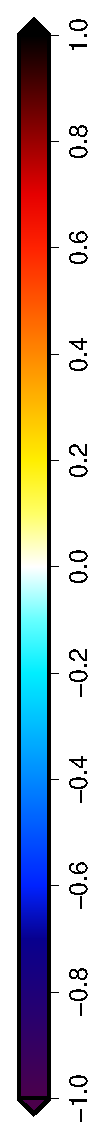
\includegraphics[height=5in,angle=270]{legends/thetaDiffWide.eps}
%
	\caption{Potential temperature anomalies of terrain following advection of a stable potential temperature profile at $t = \SI{18000}{\second}$.}
	\label{fig:wobblyThetaAdvection:thetaDiff}
\end{figure}

\begin{table}
\centering
\begin{tabular}{ r @{\hspace{2em}} l l l l l l l l}
\toprule
			& \multicolumn{3}{c}{Gravity waves, $h_0 = \SI{250}{\meter}$}	& \multicolumn{3}{c}{Gravity waves, $h_0 = \SI{500}{\meter}$}	& \multicolumn{2}{c}{Thermal profile advection} \\
Height (\si{\meter})	& BTF	& SLEVE	&	SnapCol	& BTF	& SLEVE	& SnapCol & BTF & SnapCol \\ \midrule
150 & \num{-0.003} & \num{-0.001} \\
450 & \num{0.006}  & \num{0.013} \\
750 & \num{0.032}  & \num{0.03} \\
1050 & \num{0.046} & \num{0.04} \\
\bottomrule
\end{tabular}
%
\caption{\TODO}
\label{fig:theta-sample}
\end{table}

